\documentclass{article}


\usepackage{../../austin137}
\usepackage{../../local}
\usehyperstuff

\begin{document}

%%%%%%%%%%%%%%%%%%%%%%%%%%%%%%%%%%%%%%%%%%%%%%%%%%%%%%%%%%%%%%%%%%%%%%%%%%%%%%%%
\addcopyright
\begin{center}
{\bf \large Physics W89 - Introduction to Mathematical Physics - Summer 2023}\\\medskip
{\bf \large Problem Set - Module 04 - The Matrix Squared} \\\medskip
{\emph{Last Update: \today}}
\end{center}


\dphline
\bigskip
%%%%%%%%%%%%%%%%%%%%%%%%%%%%%%%%%%%%%%%%%%%%%%%%%%%%%%%%%%%%%%%%%%%%%%%%%%%%%%%%
\section*{Problem 4.1 - Squares, Triangles, Etc.}
\relevid{Square Matrix Operations;
Classifications of Square Matrices;
The Trace}


%%%%%%%%%%%%%%%%%%%%%
\paragraph{(a)}
Show that the product of two $(2\times 2)$-upper triangular matrices is an upper triangular matrix.  \note{By transposing your result, a similar statement holds
for lower-triangular matrices.}

\begin{solution}
	Here we can just multiply two upper triangular matrices:
	\[
		\begin{pmatrix} a & b \\ 0 & c \end{pmatrix} \begin{pmatrix} d & e\\0 & f \end{pmatrix} = 
		\begin{pmatrix} ad & ae + bf \\ 0 & cf \end{pmatrix} 
	\] 
	and we can see that the result is still an upper triangular matrix, as desired. 
\end{solution}



\phline
%%%%%%%%%%%%%%%%%%%%%
\paragraph{}
Now consider the $(2\times2)$-square matrix $\mathsf{B} = \smmatrix{0.8}{z_{1} & z_{2} \\ z_{3} & z_{4}}$, where $z_{1}$ through $z_{4}$ are four complex numbers.

\paragraph{(b)}
Under what conditions on $z_{1}$ through $z_{4}$ is the matrix real?  Symmetric?  Hermitian?
Find the symmetric, antisymmetric, Hermitian, and anti-Hermitian parts of $\mathsf{B}$.  Verify that multiplying the anti-Hermitian part of $B$ by $-i$ results in a Hermitian matrix.


\begin{solution}
	Going down the list: 
	\begin{itemize}
		\item \textbf{Real:} We require that $\Im(z_i) = 0$ for all $i = 1, 2, 3, 4$.
		\item \textbf{Symmetric:} For the matrix to be symmetric we require that $B_{ij} = B_{ji}$, so therefore
			this means that $z_2 = z_3$ is the only requirement.
		\item \textbf{Hermitian:} Taking the Hermitian conjugate of $B$:
			\[
				B^\dagger = \begin{pmatrix} z_1^* & z_3^*\\ z_2^* & z_4^* \end{pmatrix} 
			\] 
			For the matrix to be Hermitian we require that $B = B^\dagger$. Comparing the terms, this means we 
			require the conditions: $\Im(z_1) = \Im(z_4) = 0$, and $z_2 = z_3^*, z_3 = z_2^*$.
	\end{itemize}
	Let's first start by finding the symmetric and antisymmetric parts. We know from lecture that 
	\[
		A_{\text{sym}} = \frac{A + A^\T}{2} \phantom{aaaa} A_{\text{anti-sym}} = \frac{A - A^\T}{2}
	\] 
	So therefore:
	\begin{align*}
		B_{\text{sym}} &= \frac{1}{2}\left[ \begin{pmatrix} z_1 & z_2\\ z_3 & z_4 \end{pmatrix} + \begin{pmatrix} z_1 & z_3 \\ z_2 & z_4 \end{pmatrix}\right] \\
					   &= \frac{1}{2}\begin{pmatrix} 2z_1 & z_2 + z_3\\ z_2 + z_3 & 2z_4\end{pmatrix} \\
					   &= \begin{pmatrix} z_1 & (z_2 + z_3)/2\\ (z_2 + z_3) / 2 & z_4 \end{pmatrix} 
	\end{align*} 
	Likewise: 
	\begin{align*}
		B_{\text{anti-sym}} &= \frac{1}{2}\left[ \begin{pmatrix} z_1 & z_2\\ z_3 & z_4 \end{pmatrix} -
		\begin{pmatrix} z_1 & z_3 \\ z_2 & z_4 \end{pmatrix}\right] \\
							&= \frac{1}{2}\begin{pmatrix} 0 & z_2 - z_3\\ z_3 - z_2& 0 \end{pmatrix}  \\
							&= \begin{pmatrix} 0 & (z_2 - z_3) / 2 \\ (z_3 - z_2) / 2 & 0\end{pmatrix}
	\end{align*}
	As for the Hermitian and anti-Hermitian parts, we also have a formula: 
	\[
		A_{\text{Herm}} = \frac{A + A^\dagger}{2} \phantom{aaa} A_{\text{anti-Herm}} = \frac{A - A^\dagger}{2}
	\] 
	So, applying these formulas:
	\begin{align*}
		B_{\text{Herm}} &= \frac{1}{2}\left[\begin{pmatrix} z_1&z_2\\z_3 & z_4 \end{pmatrix} + 
		\begin{pmatrix} z_1^* & z_3^*\\ z_2^* & z_4^* \end{pmatrix}\right]  \\
			&= \frac{1}{2}\begin{pmatrix} z_1 + z_1^* & z_2 + z_3^*\\ z_3 + z_2^* & z_4 + z_4^* \end{pmatrix}  \\
	\end{align*} 
	Here we can then use the identity $\Re(z) = \frac{z + z^*}{2}$ to simplify the diagonal elements:
	\[
		B_{\text{Herm}} = \begin{pmatrix} \Re(z_1) & (z_2 + z_3^*)/2\\ (z_3 + z_2^*) / 2 & \Re(z_4) \end{pmatrix} 
	\] 
	Now for the anti-Hermitian matrix:
	\begin{align*}
		B_{\text{anti-Herm}} &= \frac{1}{2}\left[\begin{pmatrix} z_1&z_2\\z_3 & z_4 \end{pmatrix} - 
		\begin{pmatrix} z_1^* & z_3^*\\ z_2^* & z_4^* \end{pmatrix}\right] \\
							  &= \frac{1}{2}\begin{pmatrix} z_1 - z_1^* & z_2 - z_3^* \\ z_3 - z_2^* &
							  z_4 - z_4^*\end{pmatrix}
	\end{align*}
	And again, we now use the identity $i \Im (z) = \frac{z - z^*}{2}$ to simplify the diagonal elements:
	\[
		B_{\text{anti-Herm}} = \begin{pmatrix} i\Im(z_1) & (z_2 - z_3^*) / 2\\ (z_3 - z_2^*) / 2 & i\Im(z_4)
		\end{pmatrix} 
	\] 
	Multiplying this by $-i$:
	\[
		-iB_{\text{anti-Herm}} = \begin{pmatrix} \Im(z_1) & -i(z_2 - z_3^*)/2\\ -i(z_3 - z_2^*) / 2 & \Im(z_4) 
		\end{pmatrix} 
	\] 
	Now to verify that this is Hermitian, let's take the Hermitian conjugate of this. Remember that $\Im(z_1)$
	and $\Im(z_4)$ are both real numbers, so they equal their complex conjugate. For the off diagonal elements, 
	notice:
	\begin{align*}
		\left( \frac{-i(z_2 - z_3^*)}{2}\right)^* &= \frac{i}{2}(z_2 - z_3^*)^* = \frac{i}{2}(z_2^* - z_3) = 
	-\frac{i}{2}(z_3 - z_2^*) \\
		\left(\frac{-i(z_3 - z_2^*)}{2}\right)^* &= \frac{i}{2}(z_3 - z_2^*)^* = \frac{i}{2}(z_3^* - z_2) = 
		-\frac{i}{2}(z_2 - z_3^*)
\end{align*} 
	Meaning that the conjugate of one off diagonal element is equal to the other. This is convenient, since 
	when taking the Hermitian conjugate we conjugate these two off diagonal elements and swap them with one 
	another, and since their conjugate is equal to the other it means that after swapping the matrix will be
	identical. Therefore:
	\[
		(-iB_{\text{anti-Herm}})^\dagger = \begin{pmatrix} \Im(z_1) & -i(z_2 - z_3^*)/2\\ -i(z_3 - z_2^*) / 2 & \Im(z_4) 
		\end{pmatrix}
	\]
	Hence we've verified that multiplying the anti-Hermitian part by $-i$ we get a Hermitian matrix. 
\end{solution}
\phline
%%%%%%%%%%%%%%%%%%%%%
\paragraph{(c)}
Show that the trace is a \emph{linear} function from the space of $(n\times n)$-matrices to the scalars.  
That is, $\tr(c_{1}\mathsf{A}_{1}+c_{2}\mathsf{A}_{2}) = c_{1}\tr(\mathsf{A}_{1})+c_{2}\tr(\mathsf{A}_{2})$.  
Then show that $\tr(\mathsf{A}\mathsf{B}) = \tr(\mathsf{B}\mathsf{A})$.
\extrasubpart{
Show the \heavydef{cyclic property} of the trace, given a set of $p$ $(n\times n)$-matrices $\{\mathsf{A}_{1},\cdots \mathsf{A}_{p}\}$ then the trace of the product 
is invariant under cyclic permutations of the factors,\footnote{A cyclic permutation is just taking the last however-many entries and making them the first 
(``cycling'' the last element to the first element repeatedly), so the cyclic permutations of $abcde$ are $abcde$, $bcdea$, $cdeab$, $deabc$, and $eabcd$.}
	$\tr(\mathsf{A}_{1}\mathsf{A}_{2}\cdots \mathsf{A}_{p}) = \tr(\mathsf{A}_{p}\mathsf{A}_{1}\cdots \mathsf{A}_{p-1}) 
		= \tr(\mathsf{A}_{p-1}\mathsf{A}_{p}\mathsf{A}_{1}\cdots \mathsf{A}_{p-2}) = \cdots.$}

\begin{solution}
	First let's prove the linearity condition. Let the matrices be represnted as follows: 
	\[
		A_1 = \begin{pmatrix} a_{11} & \cdots & a_{1n}\\ \vdots & \ddots & \vdots\\ a_{n 1} & \cdots &  a_{nn}
			\end{pmatrix} \phantom{aaaa} 
			A_2 = \begin{pmatrix} b_{11}& \cdots & b_{1n}\\ \vdots & \ddots & \vdots\\ b_{n 1} & \cdots & b_{nn} 
			\end{pmatrix} 
	\]
	Then we can write $c_1A_1 + c_2A_2$ as:
	\[
	c_1A_1 + c_2A_2 =\begin{pmatrix} c_1a_{11} & \cdots & c_1a_{1n}\\ \vdots & \ddots & \vdots\\ 
		c_1 a_{n 1} & \cdots & c_1 a_{nn}
			\end{pmatrix}  + \begin{pmatrix} c_2b_{11}& \cdots & c_2b_{1n}\\ \vdots & \ddots & \vdots\\ c_2 b_{n 1} & \cdots &c_2 b_{nn} 
			\end{pmatrix}  = 
		\begin{pmatrix} c_1a_{11} + c_2b_{11} & \cdots & c_1a_{1n} + c_2b_{1n}\\
		\vdots & \ddots & \vdots \\
	c_1a_{n 1} + c_2b_{n 1} & \cdots & c_1 a_{nn} + c_2 b_{nn}\end{pmatrix} 
	\] 
	Now taking the trace of this, we get: 
	\begin{align*}
		\tr(c_1A_1 + c_2A_2) &= c_1a_{11} + c_2b_{11} + c_1a_{22} + c_2b_{22} + \dots + c_1a_{nn} + c_2b_{nn}\\
							 &= c_1(a_{11} + a_{22} + \dots + a_{nn}) + c_2(b_{11} + b_{22} + \dots + b_{nn})\\
							 &= c_1\tr(A_1) + c_2\tr(A_2)
	\end{align*} 
	Now we show that $\tr(AB) = \tr(BA)$. We can define $\tr(AB)$ in index notation in the following way: 
	\[
		\tr(AB) = \sum_i(AB)^i_j \delta_{ij} = \sum_i \sum_k A^i_k B^k_j \delta_{ij} = \sum_i \sum_k A^i_k 
		B^k_i
	\] 
	Now we can also do the same for $\tr(BA)$:
	\[
		\tr(BA) = \sum_i (BA)^i_j \delta_{ij} = \sum_i \sum_k B^i_k A^k_j \delta_{ij} = \sum_i \sum_k B^i_k A^k_i
	\] 
	And since both these equations are the same, we can then conclude that $\tr(AB) = \tr(BA)$. 
\end{solution}




\bigskip
\dphline
\pagebreak
%%%%%%%%%%%%%%%%%%%%%%%%%%%%%%%%%%%%%%%%%%%%%%%%%%%%%%%%%%%%%%%%%%%%%%%%%%%%%%%%
\section*{Problem 4.2 - All About Determinants!}
\relevid{The Matrix Determinant;
Definition of the Determinant; 
Properties of the Determinant;
CramerÕs Rule;
The Wronskian}


%%%%%%%%%%%%%%%%%%%%%
\paragraph{(a)}
Find\footnote{Pun/Cryptic Spoiler: 
\spoilertext{Note that \emph{The Hitchhikers Guide to the Galaxy} is a work of fiction, so we can't just claim that 42 is the real answer.}\footnotemark}
the determinant $\det \smmatrix{0.8}{1 & 2i & -3 \\ -4i & 5 & -6i \\ 7i & -8 & i}$.
\footnotetext{Spoiler: \spoilertext{Yes, yes, that was a tortured pun about the answer being $42i$.}}  
\extrasubpart{Verify that using the Laplace exampsion on the first row to find the determinant from part (b) gives the same answer as 
using it on the 2nd column.}

\begin{solution}
	We can just run through the determinant:
	\begin{align*}
		\det \begin{pmatrix} 1 & 2i & -3\\ -4i & 5 & -6i\\7i & -8 & i \end{pmatrix} &= 1 \begin{vmatrix} 
		5 & -6i \\ -8 & i\end{vmatrix} - 2i \begin{vmatrix} -4i & -6i \\ 7i & i\end{vmatrix} + (-3) 
		\begin{vmatrix} -4i & 5 \\ 7i & -8 \end{vmatrix}\\ 
							&= 5i - 48i - (2i)(4 - 42) + (-3)(32i  - 35i)\\
							&= 42i
	\end{align*}
\end{solution}

%%%%%%%%%%%%%%%%%%%%%
\paragraph{(b)}
Use a proof by induction and the Laplace expansion method of finding determinants to show that the determinant of an upper triangular matrix is just the product of the
diagonal elements.\footnote{See the problem set supplement to Module 1 for a review of proof by induction.}  
That is, start by showing the statement is true for $(1\times 1)$-matrices.\footnote{It will be trivially true here.}  Then, \emph{assume}
that the statement is true for $(k\times k)$-upper triangular matrices and show that the statement is true for $((k+1)\times(k+1))$-upper triangular matrices.
\spoilers{Use the first column (which contains lots and lots of zeros) in our recursive way of finding determinants.}\\
\note{By using the transpose you can use this result to prove the same statement about lower-triangular matrices.}

\begin{solution}
	First we show the statement is true with 1x1 matrices. This is fairly trivial:
	\[
	\det((a)) = a
	\] 
	and since $a$ is the only value on the diagonal, the base case is verified. Now we assume that this property
	holds for $k \times k$ matrices. Now we prove that it's true also for $(k+1) \times (k+1)$ sized
	matrices. Writing out the determinant for such a matrix, call it $A$:
	\[
		\det(A) = \det\begin{pmatrix} a_{11} & a_{12} & \dots & a_{1 (k+1)}\\
		0 & a_{22} & \dots \\
	\vdots & & \ddots & \vdots\\
0 & 0 & \dots & a_{(k+1) (k+1)}\end{pmatrix}
	\]	
	Now we'll just use the first column, which has all zeroes except for the first term, so the determinant
	will just be given by that first term. Thus:
	\[
		\det(A) = a_{11} \begin{vmatrix} a_{22} & \dots & a_{2 (k+1)}\\ 0 & a_{33} & \dots  \\
			\vdots & \ddots & \vdots\\
		0  & \dots & a_{(k+1) (k+1)}\end{vmatrix}
	\] 
	But notice here that this determinant is a $k\times k$ sized upper
	triangular matrix, so we know from our inductive hypothesis that this 
	determinant actually evaluates to just the product of the 
	diagonal. Then we multiply this by $a_{11}$ out in front: 
	\[
		\det(A) = a_{11}a_{22} \dots a_{(k+1)(k+1)}
	\]
	which is exactly the product along the diagonal of our original 
	$(k+1) \times (k+1)$ matrix, as desired. 
\end{solution}

\phline
%%%%%%%%%%%%%%%%%%%%%
\paragraph{\ul{Volume:}}
\heavydef{Parallelepipeds} are the higher-dimensional versions of parallelograms.  For three dimensions, this could look like a skewed rectangular box.
The signed volume of a parallelepiped is the determinant of the set of $n$ vectors that define the edges of the parallelepiped.\footnote{By ``signed'' here we mean that the sign of the volume 
indicates the orientation, which is related to right-hand rules and such.}
The volume of a tetrahedron generated by three vectors $\vec{A},\vec{B},\vec{C}$ is one-sixth the volume of the parallelepiped created by the same vectors, so
	\begin{equation*}
		\textrm{Vol(tetrahedron)} = \fracsm{1}{6} \det\begin{pmatrix}\vec{A}&\vec{B}&\vec{C}\end{pmatrix}.
	\end{equation*}
Consider the tetrahedron generated by the vectors $\vec{A} = \hat{y} + \hat{z}$, $\vec{B} = \hat{x}+\hat{z}$, and $\vec{C} = \hat{x}+\hat{y}$, as shown.
	%~~~~~~~~~~~~~~ FIGURE ~~~~~~~~~~~~~~%
	\begin{center}	
		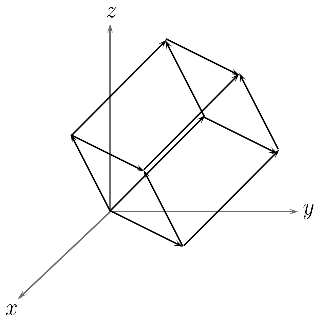
\includegraphics[width = .3\textwidth]{89-PS4-P2-Parallelepiped}	\qquad\qquad 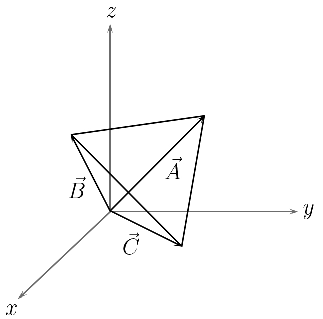
\includegraphics[width = .3\textwidth]{89-PS4-P2-Tetrahedron}
	\end{center}
	%~~~~~~~~~~~~~~ FIGURE ~~~~~~~~~~~~~~%


\paragraph{(c)}
Use the determinant to find the volume of the tetrahedron!  
\\\note{If you would like, you can check your answer by using the formula $\textrm{Volume} = \fracsm{1}{6}\,\vec{A}\bcdot(\vec{B}\times\vec{C})$.}

\begin{solution}
	Noting that $\vec A = \begin{pmatrix} 0 \\ 1\\1 \end{pmatrix}, \vec B = \begin{pmatrix} 1 \\ 0\\1
	\end{pmatrix}$ and $\vec C = \begin{pmatrix} 1 \\ 1\\0 \end{pmatrix}$, we can now build the 
	quantity $(\vec A \ \ \vec B \ \ \vec C)$:
	\[
		(\vec A \ \ \vec B \ \ \vec C) = \begin{pmatrix} 0 & 1 & 1 \\ 1 & 0 & 1\\ 1 & 1 & 0 \end{pmatrix} 
	\] 
	So now we can take the determinant of this:
	\[
		\det (\vec A \ \vec B \ \vec C) = - 1 \begin{vmatrix} 1 & 1 \\ 1 & 0 \end{vmatrix} + 1 
		\begin{vmatrix} 1 & 0 \\ 1 & 1 \end{vmatrix} = 1 + 1 = 2
	\] 
	Then we divide this by 6 according to the formula, so the volume of the tetrahedron is going to be
	$\frac{1}{3}$.

\end{solution}

\phline
%%%%%%%%%%%%%%%%%%%%%
\paragraph{\ul{Coordinate Changes:}}
Consider two coordinate systems for a space (for example, the Cartesian coordinates $(x,y)$ and
polar coordinates $(r,\theta)$ for the plane).  The \heavydef{Jacobian} for a transformation from coordinates $(x_{1},\cdots,x_{n})$ to coordinates
$(u_{1},\cdots,u_{n})$ is defined as\footnote{We will be introduced to the Jacobian more formally in Module 7.} 
	\begin{subequations}
	\begin{equation}
		J \equiv \det\begin{smpmatrix}{0.8}\fracsm{\partial{x_{1}}}{\partial{u_{1}}}&\cdots&\fracsm{\partial{x_{1}}}{\partial{u_{n}}}\\\vdots&\ddots&\vdots\\
		\fracsm{\partial{x_{n}}}{\partial{u_{1}}}&\cdots&\fracsm{\partial{x_{n}}}{\partial{u_{n}}}\end{smpmatrix}.
	\label{jacob}
	\end{equation}
The Jacobian provides a relationship between the volume elements for the two coordinate systems,\footnote{This is very tied in with the fact that the determinant
gives the volume of a parallelepiped!}
	\begin{equation}
		dx_{1}\cdots dx_{n} = \abs{J}\,du_{1}\cdots du_{n}.
	\label{volumes}
	\end{equation}
	\end{subequations}
For spherical coordinates in three dimensions,
	\begin{equation*}
		\smthreevect{x}{y}{z} = \smthreevect{r\sin\theta\cos\varphi}{r\sin\theta\sin\varphi}{r\cos\theta},
	\end{equation*}
where $\theta$ is the polar angle and $\varphi$ is the azimuthal angle.\footnote{This is the physics convention for angles in spherical coordinates.  The math convention
is the opposite.}  The angle $\theta$ ranges from 0 to $\pi$ and the angle $\varphi$ ranges from 0 to $2\pi$.

%%%%%%%%%%%%%%%%%%%%%
\paragraph{(d)}
Find the Jacobian for the transformation from Cartesian coordinates $(x,y,z)$ to spherical coordinates $(r,\theta,\varphi)$.  Simplify until you get a result that is independent of
$\varphi$.  Use your result to find the volume of a sphere of radius $R$.
\spoilers{The volume is initially given by an integral in Cartesian coordinates as $V = \iiint_{\textrm{sphere}} dx\,dy\,dz$.  Use your Jacobian to rewrite the
volume element in spherical coordinates, then put in the appropriate integral limits for the sphere ($0 \leq \theta \leq \pi$, $0\leq \varphi \leq 2\pi$, $0\leq r \leq R$).}

\begin{solution}
	So we first identify that our $u_i$ are going to be derivatives in $r, \theta, \phi$. Therefore, 
	taking derivatives, we get the Jacobian matrix:
	\[
		J = \begin{vmatrix} \sin \theta \cos \phi & r \cos \theta \cos \phi & - r \sin \theta \sin \phi\\ 
		\sin \theta \sin \phi & r \cos \theta \sin \phi & r \sin \theta \cos \phi\\
	\cos \theta & - r \sin \theta & 0\end{vmatrix}
	\]
	This determinant then evaluates to:
	\begin{multline*}
		J = \sin \theta \cos \phi(-r \sin \theta \cos \theta(-r \sin \theta)) 
		-r \cos \theta \cos \phi(-r \sin \theta \cos \phi \cos \theta) \\
		-r \sin \theta \sin \phi (\sin \theta \sin \phi(-r \sin \theta) - r \cos \theta \sin \phi \cos \theta)
	\end{multline*}
	Simplifying:
	\begin{align*}
	J &= \sin \theta \cos \phi(r^2 \sin^2 \theta \cos \phi) - r \cos \theta \cos \phi(-r \sin \theta \cos \phi 
	\cos \theta) - r \sin \theta \sin \phi(\underbrace{-r \sin^2 \theta \sin \phi - r \cos^2 \theta \sin \phi}_
	{= -r \sin \phi (\sin^2 \theta + \cos^2 \theta) = -r \sin \phi})\\
	&= r^2 \sin^3 \theta \cos^2\phi + r^2 \cos^2 \theta \cos^2 \phi \sin \theta + r^2 \sin \theta \sin^2 \phi \\
	&= r^2 \sin \theta \left( \sin^2 \theta \cos^2 \phi + \cos^2 \theta \cos^2 \phi + \sin^2 \phi\right) \\
	&= r^2 \sin \theta \left( \cos^2 \phi (\sin^2 \theta + \cos^2 \theta) + \sin^2 \phi \right)  \\
	&= r^2 \sin \theta(\cos^2 \phi + \sin^2 \phi) \\
	&= r^2 \sin \theta 
		\end{align*} 
	To find the volume, normally when we would write $dx dy dz$, now we write $|J| dr d\theta d\phi$. Now for 
	a sphere of radius $R$, then $r$ goes from 0 to $R$, $\theta$ goes from 0 to $\pi$ and $\phi$ goes from 
	0 to $2\pi$. Therefore:
	\begin{align*}
		V &= \int_0^{2\pi} \int_0^\pi \int_0^R r^2 \sin \theta dr d\theta d\phi\\ 
		&= 2\pi \int_0^R r^2 dr \int_0^\pi \sin \theta d\theta \\
		&= 2\pi \left(\frac{R^3}{3}\right)(\pi) \\
		&= \frac{4\pi R^3}{3} 
	\end{align*} 
	which is the correct formula for the volume of a sphere. 
\end{solution}


\phline
%%%%%%%%%%%%%%%%%%%%%
\paragraph{\ul{Linear Independence of Vectors:}}
Determinants provide a great way of determining lthe linear independence of a set of vectors!
In lecture, we defined the determinant of a set of $n$ vectors $\{\vec{a}_{i}\}$ in an $n$-dimensional vector space to be the object that satisfied the properties of 
linearity in each entry, antisymmetry, and normalization.  If we create the $(n\times n)$-matrix $\mathsf{A}=\begin{pmatrix}\vec{a}_{1}&\cdots&\vec{a}_{n}\end{pmatrix}$
using the vectors $\{\vec{a}_{i}\}$ as the column vectors, than the determinant of vectors equals the matrix determinant of $\mathsf{A}$.

\paragraph{}
Suppose we have a linearly \emph{dependent} set of vectors $\{\vec{a}_{i}\}$, so we can write one of them as a linear combination
of the others.  (For concreteness, let the last vector $\vec{a}_{n}$ be some linear combination of the first $n-1$ vectors - if it is not we can always flip our columns 
using the antisymmetry property of the determinant so that this is true without affecting the proof!)

\paragraph{(e)}
Prove that in this case we must have $\det \mathsf{A} = 0$.

\begin{solution}
	I'll also use the fact that $\vec a_n$ can be written as a linear combination of the first $n-1$ vectors. To
	start, this means that we can write: 
	\[
		\vec a_n = \sum_{k=1}^{n-1} c_k \vec a_k
	\] 
	for some constants $c_k$. Now we use the fact that the determinant is linear in each input slot. That is,
	\[
		\det(\dots, c_i\vec a_{i} + c_{j}\vec a_{j}, \dots) = c_i \det(\dots, \vec a_i, \dots) +
		c_{j}\det(\dots, \vec a_{
		j}, \dots)
	\] 
	Essentially, this means that if one of the entries can be written as a linear combination of two 
	other vectors, then we can apply this rule to ``split'' them up. Now, if $\vec a_n$ can be written 
	as a linear combination of the first $n-1$ entries, this means that we can write:
	\begin{align*}
		\det(\vec a_1, \dots, \sum_{k=1}^{n-1} c_k \vec a_k) &= \sum_{k = 1}^k c_k \det(\vec a_1, \dots, \vec a_k)
	\end{align*}
	Then, since we know that each $\vec a_k$ is another vector in $\{a_1, \dots, a_{n-1}\}$, then this means 
	that in all these determinants, we have two identical columns in the determinant, which we already know 
	amounts to a value of zero. 

	To add to this, even if the component of $\vec a_n$ along some $\vec a_k$ is zero, this would imply that 
	$c_k = 0$, which gives us zero anyways, regardless of what the determinant is. The determinant would
	nonetheless give us zero because there are two identical rows, but this is something else we can derive from
	the problem.
\end{solution}

\phline
%%%%%%%%%%%%%%%%%%%%%
\paragraph{}
Since $\det{\mathsf{A}^{\T}} = \det \mathsf{A}$, anything we say about columns and determinants \emph{also} applies to rows.  

\paragraph{(f)}
Determine what each of the three row-reduction operations (flipping a pair of rows, multiplying a row by a non-zero scalar, adding a multiple of one row to another)
does to the determinant of a matrix.

\begin{solution}
	For all the row operations, because we know that $\det(A) = \det(A^\T)$, we can instead rephrase these 
	questions in terms of column operations instead. Now, we use the properties of the matrix determinant. 

	Firstly, we know that the matrix determinant is antisymmetric. That is, using the vector space 
	definition of the determinant:
	\[
	\det(\dots, \vec v_i, \vec v_j, \dots) = -\det(\dots, \vec v_j, \vec v_i, \dots)
	\] 
	And this holds true for any two vectors $\vec v_i, \vec v_j$ we choose. Therefore, if we swap two columns,
	this means that the sign of the determinant must flip. This holds true also if we swap two rows.

	We also know that the determinant is linear in its inputs. That is:
	\[
	\det(\dots, c_i\vec v_i, \dots) = c_i \det(\dots, \vec v_i, \dots) 
	\] 
	What this means is that if we scale a column by a non-zero scalar, we just multiply the original (the 
	the determinant where the column was not scaled) by that scaling constant. The same applies to rows, so when
	we multiply a row by a nonzero scalar we can take that scalar out and multiply it to the remaining
	determinant. 

	Finally, we use linearity again:
	\[
	\det(\dots, \vec w_1 + c_2 \vec w_2, \dots) = \det(\dots, \vec w_1, \dots) + 
	c_2 \det(\dots, \vec w_2, \dots)
	\] 
	For the sake of argument, let's say that $c_2 \vec w_2$ is being added to the column containing $\vec w_1$.
	Then, this equation
	says that this is equal to the original determinant, plus the original determinant except with $\vec w_2$
	replacing where $\vec w_1$ used to be and multiplying by that scale factor $c_2$. However, notice that 
	$\vec w_2$ must also exist as a column somewhere else in the determinant, since we scaled by a constant
	times \textit{another column in the determinant}. Hence, this second determinant has two copies of 
	$\vec w_2$, and we know that when a determinant has two identical rows, its value is zero. Therefore, 
	the determinant actually remains unchanged. 

	The same argument applies to rows, so adding a multiple of one row to another doesn't change the value of 
	the determinant. 
\end{solution}

%%%%%%%%%%%%%%%%%%%%%
\paragraph{(g)}	\extrapart
Let $\mathsf{A}_{rr}$ be the reduced row echelon form of $\mathsf{A}$ and use the results from previous parts to show that $\det{\mathsf{A}}\neq 0$ only if 
$\det{\mathsf{A}_{\textrm{rr}}}\neq 0$.
\extrasubpart{Argue that the only way for a matrix $\mathsf{A}$ to have a  non-zero determinant is if it reduces to the identity matrix, $A_{\textrm{rr}} = \mathbbold{1}$.}


%%%%%%%%%%%%%%%%%%%%%
\paragraph{}
\noindent\textit{Commentary: As a result of these parts we can conclude a lot of things! Let $A:V\to V$ be an automorphism 
and let $\mathsf{A}$ be the matrix representation of $A$ with respect to some basis.  If $\det{A} \neq 0$, then...
	\begin{itemize}
		\item The column vectors of $\mathsf{A}$ are linearly independent (as are the row vectors)! 
		\item $\rank A = \dim V$ and $\nullity A = 0$.
		\item The linear transformation $A$ is one-to-one ($\ker{A} = \{\vec{0}\}$) and onto ($\Im{A} = V$) and thus
		$A$ is an isomorphism/is bijective/is invertible.
		\item The equation $A\vec{x} = \vec{b}$ always has a unique solution. 
	\end{itemize}}

\phline
%%%%%%%%%%%%%%%%%%%%%
\paragraph{\ul{Linear Independence of Functions:}}
Consider the three functions $\{e^{\lambda_{1}x},e^{\lambda_{2}x}, e^{\lambda_{3}x}\}$, with the three $\lambda$s distinct.

\paragraph{(h)}	
Use the \heavydef{Wronskian} to show that these three functions are linearly independent.

\begin{solution}
	The Wronskian matrix is then: 
	\[
		\mathbb W = \begin{pmatrix} e^{\lambda_1 x} & e^{\lambda_2x} & e^{\lambda_3x}\\
		\lambda_1 e^{\lambda_1x} & \lambda_2e^{\lambda_2x} & \lambda_3e^{\lambda_3x}\\
	\lambda_1^2 e^{\lambda_1x} & \lambda_2^2 e^{\lambda_2x} & \lambda_3^2e^{\lambda_3x}\end{pmatrix} 
	\] 
	So now we take the determinant
	\begin{multline*}
		\det(\mathbb W) = e^{\lambda_1x}\left( \lambda_2\lambda_3^2 e^{(\lambda_2 + \lambda_3)x} - \lambda_3\lambda_2^2
			e^{(\lambda_2 + \lambda_3)x}\right) + 
			e^{\lambda_2x} \left( \lambda_1 \lambda_3^2 e^{(\lambda_1 + \lambda_3)x} - \lambda_3\lambda_1^2
		e^{(\lambda_1 + \lambda_3)x}\right) \\
		+ e^{\lambda_3 x}\left(\lambda_1\lambda_2^2 e^{(\lambda_1 + \lambda_2)x} - 
			\lambda_2\lambda_1^2 e^{(\lambda_1 + \lambda_2)x}\right)
	\end{multline*}
	Simplifying:
	\begin{align*}
		\det(\mathbb W) &= e^{\lambda_1x}e^{(\lambda_2 +\lambda_3)x}\left( \lambda_2\lambda_3^2 - 
		\lambda_3\lambda_2^2\right) + e^{\lambda_2x} e^{(\lambda_1 + \lambda_3)x} \left( \lambda_1\lambda_3^2 -
		\lambda_3\lambda_1^2\right) + e^{\lambda_3x}e^{(\lambda_1 + \lambda_2)x}\left( \lambda_1 \lambda_2^2 - 
			\lambda_2 \lambda_1^2\right)\\
		&= e^{(\lambda_1 + \lambda_2 + \lambda_3)x} \left[ \lambda_2\lambda_3(\lambda_3 - \lambda_2) + 
		\lambda_1 \lambda_3(\lambda_3 - \lambda_1) + \lambda_1 \lambda_2(\lambda_2 - \lambda_1)\right]
	\end{align*}
	If the three $\lambda$s are distinct, then at most one of them is zero, but this would always leave 
	one of the terms unaffected, since each individual term only contains two of the three $\lambda$s. 
	Specifically, the term that is unaffected will be the one that doesn't contain that particular $\lambda$
	that equals zero. This would still guarantee that the Wronskian is always nonzero, since this means
	there will be at least one nonzero term, and $e^{(\lambda_1 + \lambda_2 + \lambda_3)x}$ is never zero 
	since it's an exponential function. So in the end, we will have an exponential (nonzero) multiplied with 
	the square brackets (also nonzero), which will always result in a nonzero number. 

	Thus, we conclude that these three functions are linearly independent. 
\end{solution}
\bigskip
\dphline
\pagebreak
%%%%%%%%%%%%%%%%%%%%%%%%%%%%%%%%%%%%%%%%%%%%%%%%%%%%%%%%%%%%%%%%%%%%%%%%%%%%%%%%
\section*{Problem 4.3 - The Matrix Inverse}
\relevid{Introduction to the Matrix Inverse;
Constructing the Matrix Inverse;
Properties of the Matrix Inverse}

%%%%%%%%%%%%%%%%%%%%%
\paragraph{}
Recall that the matrix inverse for a square matrix $M$ (or an automorphism $\mathsf{M}$ mapping a space to itself)
is defined via $\mathsf{M}^{-1}\mathsf{M}=\mathsf{MM}^{-1} = \mathbbold{1}$ and only exists if $\det \mathsf{M} \neq 0$.  
We have two main ways of computing matrix inverses:  
	\begin{itemize}
	\item Row reduction (also called Gauss-Jordan elimination):
	\begin{equation*}
		\begin{amatrix}{1} \scalebox{1.1}{$\mathsf{A}$\vphantom{$\mathsf{A}^{-1}$}} & \scalebox{1.2}{$\mathbbold{1}$}\end{amatrix}	
		\quad \xrightarrow{\textrm{Row reduces to}}	\quad
		\begin{amatrix}{1} \scalebox{1.2}{$\mathbbold{1}$} & \scalebox{1.1}{$\mathsf{A}^{-1}$}\end{amatrix}.
	\end{equation*}
	\item Using the cofactor matrix $\mathsf{C}_{A}$,
		\begin{equation*}
			\mathsf{A}^{-1} = \frac{\mathsf{C}_{A}^{\T}}{\det \mathsf{A}}.
		\end{equation*}
	\end{itemize}

\phline	
%%%%%%%%%%%%%%%%%%%%%
\paragraph{(a)}
First use \emph{row reduction} to solve for the inverse of the matrix $\mathsf{B} = \smmatrix{0.7}{1 & 0 & 1\\2 & 1 & 1 \\ 2 & 1 & 2}$.  
Be sure to explain your steps and \ul{explicitly verify} that you have found the inverse by computing $\mathsf{B}^{-1}\mathsf{B}$.

\begin{solution}
	So we start off with the matrix:
	\[
		\begin{pmatrix} 1 & 0& 1& 1 &0&0\\2&1&1&0&1&0\\2&1&2&0&0&1 \end{pmatrix} 
	\] 
	First, we subtract row 2 from row 3:
	\[
		\begin{pmatrix} 1&0&1&1&0&0\\2&1&1&0&1&0\\0&0&1&0&-1&1 \end{pmatrix} 
	\] 
	Now subtract 2 times row 1 from row 2($R_2 - 2R_1$):
	\[
		\begin{pmatrix} 1&0&0&1&1&-1\\0&1&0&-2&0&1\\0&0&1&0&-1&1 \end{pmatrix} 
	\] 
	Now we subtract row 3 from row 1, and add row 3 to row 2:
	\[
		\begin{pmatrix} 1&0&0&1&1&-1\\0&1&0&-2&0&1\\0&0&1&0&-1&1 \end{pmatrix} 
	\] 
	The first three columns are now the identity matrix, meaning that the latter three columns are the inverse: 
	\[
		B^{-1} = \begin{pmatrix} 1&1&-1\\-2&0&1\\0&-1&1 \end{pmatrix} 
	\] 
	To explicitly show that the inverse is what we computed, let's do the matrix multiplication: 
	\begin{align*}
		B^{-1}B &= \begin{pmatrix} 1&1&-1\\-2&0&1\\0&-1&1 \end{pmatrix} 
		\begin{pmatrix} 1&0&1\\2&1&1&\\2&1&2 \end{pmatrix} \\
						 &= \begin{pmatrix} (1)(1) + (1)(2) + (1)(-2)& (1)(0)+ (1)(1)+ (-1)(1)& 
						 (1)(1) + (1)(1) + (1)(-2)\\
					 (-2)(1) + (0)(2) + (1)(2) & (-2)(0) + (0)(1) + (1)(1) & (-2)(1) + (0)(1) + (1)(2)\\
					 (0)(1) + (-1)(2) + (1)(2) & (0)(0) + (-1)(1) + (1)(1) & (0)(1) + (-1)(1) + (1)(2)
				 \end{pmatrix} \\
						 &= \begin{pmatrix} 1&0&0\\0&1&0\\0&0&1 \end{pmatrix} 
	\end{align*} 
	I think this is about as explicit as I can get without being unnecessary. 
\end{solution}
%%%%%%%%%%%%%%%%%%%%%
\paragraph{(b)}
Now use the \emph{cofactor matrix} to find the same inverse of the matrix $\mathsf{B} = \smmatrix{0.7}{1 & 0 & 1\\2 & 1 & 1 \\ 2 & 1 & 2}$.  
Again, explain your steps. You should obviously get the same final answer as part (a)!

\begin{solution}
	To find the cofactor matrix, we find the minors of each matrix element then insert the positives and 
	negatives later. I won't write out the entire process for my sanity, but for instance, the minor
	of the first element $b_{11}$ is:
	\[
		(m_b)^1_1 = \begin{vmatrix} 1 & 1\\1&2\end{vmatrix} = 2 - 1 = 1
	\] 
	Then for $b_{12}$:
	\[
		(m_b)^1_2 = \begin{vmatrix} 2&1\\2&2\end{vmatrix} = 4 - 2 = 2
	\] 
	But here, we need to flip the sign due to the positives and negatives we need to insert for the cofactor:
	\[
		(c_B)^1_2 = -(m_b)^1_2 = -2
	\] 
	And this process carries on all throughout the matrix. Therefore, the final cofactor matrix is:
	\[
		C_B = \begin{pmatrix} 1&-2&0\\1&0&-1\\-1&1&1 \end{pmatrix} 
	\] 
	Taking the transpose:
	\[
		C_B^\T = \begin{pmatrix} 1&1&-1\\-2&0&1\\0&-1&1 \end{pmatrix} 
	\] 
	Now we find the determinant of $B$:
	\[
	\det(B) = 1(1) - 0(-2) + 1(0) = 1
	\] 
	So therefore, the inverse is actually just the transpose of the cofactor matrix:
	\[
		B^{-1} = \begin{pmatrix} 1&1&-1\\-2&0&1\\0&-1&1 \end{pmatrix} 
	\] 
	which is exactly the matrix part (a) gives us. 
\end{solution}
\phline
%%%%%%%%%%%%%%%%%%%%%
\paragraph{}
Consider an arbitrary invertible $(3\times 3)$ lower-triangular matrix, $\mathsf{T} = \smmatrix{0.8}{a & 0 & 0\\b&c&0\\d&e&f}$.

\paragraph{(c)}
In terms of the six constants $a$ through $f$, what is the condition for this matrix to be invertible?  Use whichever method you like (row reduction or cofactors)
to find the inverse matrix $\mathsf{T}^{-1}$.

\begin{solution}
	Firstly, $T$ must be a square matrix, which $T$ satisfies. Further, the determinant of $T$ must be nonzero. 
	Given that $T$ is lower triangular, this means that the determinant is just the product of the diagonal:
	\[
	\det(T) = acf
	\] 
	So the condition essentially boils down to $a, c, f \neq 0 $. 

	I'll use the cofactor process to find the inverse. I'm just going to show a few examples of how the first
	two cofactor entries are calculated, then I'll just skip to the final matrix. So calculating $(C_T)^1_1$:
	\[
		(C_T)^1_1 = \begin{vmatrix} c & 0\\ e & f\end{vmatrix} = cf
	\] 
	Then let's now do $(C_T)^1_2$:
	\[
		(C_T)^1_2 = -\begin{vmatrix} b & 0 \\ d & f\end{vmatrix} = -bf
	\] 
	And so on. We have a negative sign out in front for $(C_T)^1_2$ since we need to alternate between positive
	and negative determinants of the minors. Just to really show that I do understand the 
	process and am simply skipping steps since it would be too much typing, let's also compute 
	$(C_T)^2_3$.
	\[
		(C_t)^2_3 = -\begin{vmatrix} a & 0 \\ d &e\end{vmatrix} = -ae
	\] 
	Now with that out of the way, here's the full cofactor matrix:
	\[
		C_T = \begin{pmatrix} cf & -bf & be-cd\\0&af&-ae\\0&0&ac \end{pmatrix} 
	\] 
	Now taking the transpose:
	\[
		C_T^\T = \begin{pmatrix} cf & 0&0\\-bf & af & 0\\be-cd & -ae & ac \end{pmatrix} 
	\] 
	The determinant of $B$ is $\det(B) = acf$ as mentioned before, so therefore we divide each matrix entry 
	by $acf$: 
	\[
		T^{-1} = \begin{pmatrix} 1/a & 0&0\\-b / ac & 1 / c &0\\(be - cd) / acf & -e / cf& 1 / f\end{pmatrix} 
	\] 

\end{solution}

%%%%%%%%%%%%%%%%%%%%%
\paragraph{(d)}		\extrapart
Argue that the cofactor matrix of a general $(n\times n)$ lower-triangular matrix will always be a upper-triangular matrix and then use this result to show that
the inverse of a lower-triangular matrix is itself a lower-triangular matrix.


\phline
%%%%%%%%%%%%%%%%%%%%%
\paragraph{}
If a matrix is orthogonal or unitary then computing the inverse is as simple as taking a transpose or Hermitian conjugate!
Consider the unitary matrix $\mathsf{U} = \fracsm{1}{\sqrt{2}}\twotwomat{1}{1}{i}{-i}$.

\paragraph{(e)}
Given the fact that $\mathsf{U}$ is unitary, write down the inverse $\mathsf{U}^{-1}$.  Explicitly verify that $\mathsf{U}$ is unitary by computing $\mathsf{UU}^{\t}$.

\begin{solution}
	Given that $U$ is unitary, then we know that $U^{\dagger} = U^{-1}$. Therefore, we compute the Hermitian
	conjugate of $U$:
	\[
		U^{\dagger} = \frac{1}{\sqrt{2} }\begin{pmatrix} 1 & -i\\1 & i \end{pmatrix} 
	\] 
	Now to verify this, we compute $U U^\dagger$:
	\[
		U U^\dagger = \frac{1}{2}\begin{pmatrix} 1 & 1\\i & -i \end{pmatrix} \begin{pmatrix} 1 & -i\\
		1 & i\end{pmatrix} = \frac{1}{2}\begin{pmatrix} 2 & 0\\0&2 \end{pmatrix} = \begin{pmatrix} 1& 0\\0&1
	\end{pmatrix} = \mathbbold 1
	\] 
	which is the identity matrix, as desired. 
\end{solution}
\phline
%%%%%%%%%%%%%%%%%%%%%
\paragraph{(f)}		
Show that the inverse of a transpose is the transpose of the inverse, $(\mathsf{A}^{\T})^{-1} = (\mathsf{A}^{-1})^{\T}$.

\begin{solution}
	We multiply both sides by $A^\T$. First, we can do the left hand side:
	\[
	 (A^\T)^{-1} A^\T = \mathbbold 1
	\] 
	This is by definition, since any matrix $A$ multiplied by its inverse returns the identity. Then for the 
	right hand side:
	\[
		(A^{-1})^\T A^\T = (A A^{-1})^\T = \mathbbold 1^\T = \mathbbold 1
	\] 
	Since multiplying both sides both return the identity, we can then conclude that the original left and 
	right hand side must also be equal to one another. 
\end{solution}
\bigskip
\dphline
\pagebreak
%%%%%%%%%%%%%%%%%%%%%%%%%%%%%%%%%%%%%%%%%%%%%%%%%%%%%%%%%%%%%%%%%%%%%%%%%%%%%%%%
\section*{Problem 4.4 - Foreshadowing Module 6}
\relevid{Square Matrix Operations;
Properties of the Matrix Inverse}


%%%%%%%%%%%%%%%%%%%%%
\paragraph{(a)}		\extrapart
Argue or show that if $\mathsf{D}$ is a diagonal matrix with diagonal entries $d_{i}$ then for any Taylor-expandable function $f(x)$, the expression $f(\mathsf{D})$ is a 
diagonal matrix with diagonal entries $f(d_{i})$.\\
\note{We did this proof in lecture, but be sure you can understand the steps and why they work!}


%%%%%%%%%%%%%%%%%%%%%
\paragraph{(b)}
Consider an invertible $(n\times n)$-matrix $\mathsf{A}$ and a square $(n\times n)$-matrix $\mathsf{B}$.  Let $p\in\mathbb{N}$ be some natural number ($p=1,2,3,\cdots$).
Show that $\mathsf{A}^{-1}\mathsf{B}^{p}\mathsf{A} = (\mathsf{A}^{-1}\mathsf{BA})^{p}$.  
From this, argue that $\mathsf{A}^{-1}f(\mathsf{B})\mathsf{A} = f(\mathsf{A}^{-1}\mathsf{BA})$, where $f(x)$ is any Taylor-expandable function and $\mathsf{A}$ is any invertible matrix.

\begin{solution}
	We can do this via induction. First let $p = 1$. Then we have the trivial equality $A^{-1}BA = A^{-1}BA$, 
	since $B^{1} = B$. Now let's assume that this is true for some $k$, we prove that it's true for $k+1$.
	That is, we assume that $A^{-1}B^kA = (A^{-1}BA)^k$, and now we show it's true for $k+1$ as well. This is 
	relatively simple, we use the right hand side:
	\begin{align*}
		(A^{-1}BA)^{k+1} &= (A^{-1}BA)^k(A^{-1}BA)\\	
						 &= A^{-1}B^k\underbrace{A A^{-1}}_{=\mathbbold{1}}BA \\
						 &= A^{-1}B^kBA \\
						 &= A^{-1}B^{k+1}A 
	\end{align*}
	which is the left hand side, as desired. 

	Now for the second part of the problem, we know that if $f$ is Taylor-expandable, this means that we 
	can write 
	\[
	f(x) = \sum_n c_n x^n
	\] 
	In other words, $f$ can be written as a (potentially infinite) polynomial with coefficients $c_n$ determined
	by derivatives of $f$. We learned this module that we can also insert a square matrix $B$ as $x$:
	\[
	f(B) = \sum_n c_n B^n
	\] 
	So now if we look at the identity we want to prove: 
	\begin{align*}
		A^{-1}f(B)A &= A^{-1} \sum_n c_n B^n A\\
					&= \sum_n c_n(A^{-1}B^nA) \\
					&= \sum_n c_n(A^{-1}BA)^n 
	\end{align*}
	And this last line is actually just $f(A^{-1}BA)$, since it's the same function $f$ (defined by the 
	coefficients $c_n$, but now with $A^{-1}BA$ as the input. 
	
\end{solution}
%%%%%%%%%%%%%%%%%%%%%
\paragraph{}
Consider the following two matrices 
	\begin{equation*}
		\mathsf{A} = \fracsm{1}{\sqrt{2}}\twotwomat{1}{1}{1}{-1},	\qquad	\mathsf{K} \equiv \twotwomat{2}{-1}{-1}{2}
	\end{equation*}
The matrix $\mathsf{A}$ is an orthogonal matrix, so $\mathsf{A}^{\T}\mathsf{A} = \mathbbold{1}$.  It turns out that the combination $\mathsf{A}^{-1}\mathsf{K}\mathsf{A}$
is a diagonal matrix.  That is, $\mathsf{A}$ \heavydef{diagonalizes} $\mathsf{K}$.

%%%%%%%%%%%%%%%%%%%%%
\paragraph{(c)}
Find $\mathsf{A}^{-1}\mathsf{K}\mathsf{A}$.  Then use the conclusions from parts (a) and (b) to find $\mathsf{A}^{-1}e^{\mathsf{K}}\mathsf{A}$.  Finally, determine
$e^{\mathsf{K}}$.\\
\note{This is a much easier way of exponentiating matrices than using the full Taylor expansion!}

\begin{solution}
	Since $A$ is an orthogonal matrix, we know that $A^\T = A^{-1}$. Therefore, we have that 
	\[
		A^{-1} = \frac{1}{\sqrt{2} }\begin{pmatrix} 1 & 1\\ 1& -1 \end{pmatrix} 
	\] 
	Now we are ready to compute $A^{-1}KA$:
	\begin{align*}
		A^{-1} KA &= \frac{1}{\sqrt{2}}\begin{pmatrix} 1 & 1 \\ 1& -1 \end{pmatrix} 
		\begin{pmatrix} 2 & -1\\ -1 & 2 \end{pmatrix} 
		\cdot \frac{1}{\sqrt{2} }\begin{pmatrix} 1 & 1 \\1 & -1 \end{pmatrix} \\
		&= \frac{1}{2}\begin{pmatrix} 1 & 1\\3& -3 \end{pmatrix} 
		\begin{pmatrix} 1 & 1\\&1 &-1 \end{pmatrix}  \\
						  &= \frac{1}{2}\begin{pmatrix} 2 & 0\\ 0 & 6 \end{pmatrix}  \\
						  &= \begin{pmatrix} 1 & 0\\0 & 3 \end{pmatrix}
	\end{align*}
	Now, to find $A^{-1}e^KA$, we use the fact that $A^{-1}f(B)A = f(A^{-1}BA)$, where $f(x) = e^x$ in this case.
	Therefore:
	\[
		A^{-1}e^KA = e^{A^{-1}KA}
	\] 
	But since $A^{-1}KA$ is a diagonal matrix, we have the nice identity that:
	\[
		f\left( \begin{pmatrix} a & &\\ & b & \\ & & c \end{pmatrix} \right) = 
		\begin{pmatrix} f(a) & &\\ & f(b) & \\ & & f(c) \end{pmatrix} 
	\] 
	In other words, because we have a diagonal matrix we have the property that a function on this matrix 
	is simply just the function acting on each of the diagonal elements. Therefore:
	\[
		A^{-1}e^K A = e^{A^{-1}KA} = \exp{\begin{pmatrix} 1 & 0 \\ 0 & 3 \end{pmatrix}} 
		= \begin{pmatrix} e & 0 \\ 0 & e^3\end{pmatrix} 
	\] 
	Now that we know this, we can first multiply this matrix by $A^{-1}$ on the right:
	\[
		A^{-1} e^K A A^{-1} = A^{-1}e^K = \begin{pmatrix} e & 0 \\ 0 & e^3 \end{pmatrix} \frac{1}{\sqrt{2} }\begin{pmatrix} 1 & 1 \\ 1 & -1 \end{pmatrix} 
	\] 
	Then we multiply by $A$ on the left:
	\begin{align*}
		A A^{-1}e^K = e^K &= \frac{1}{\sqrt{2} }\begin{pmatrix} 1 & 1 \\ 1& -1 \end{pmatrix} \begin{pmatrix} e & 0\\ 0 & e^3 \end{pmatrix} \frac{1}{\sqrt{2} }\begin{pmatrix} 1 & 1\\ 1& -1 \end{pmatrix} \\
						  &=  \frac{1}{2}\begin{pmatrix} e & e^3\\ e & -e^3 \end{pmatrix}\begin{pmatrix} 1 & 1 \\ 1& -1 \end{pmatrix} \\
						  &= \frac{1}{2}\begin{pmatrix} e + e^3 & e - e^3\\ e - e^3 & e + e^3 \end{pmatrix} 
	\end{align*} 
\end{solution}

\endofhomework
\addfooter
%%%%%%%%%%%%%%%%%%%%%%%%%%%%%%%%%%%%%%%%%%%%%%%%%%%%%%%%%%%%%%%%%%%%%%%%%%%%%%%%
\end{document}




